
% ============================================================
% Results and Discussion revised for Engineering Applications
% of Artificial Intelligence (EAAI)
% ============================================================
% Required packages:
% \usepackage{booktabs}
% \usepackage{longtable}
% \usepackage{array}
% \usepackage{graphicx}
% \usepackage{subcaption}
% \usepackage{placeins}
% \usepackage{threeparttable}
% \usepackage{microtype}
%
% Terminology used in this revision:
%   - "adaptive conformal uncertainty estimation"
%   - "non-stationary dynamics"
%   - "volatility-responsive gate"
%   - "Industrial Construction-Materials Demand (ICMD)"
%
% The bracketed stationarity diagnostics in Table~\ref{tab:icmd_diagnostics}
% must be populated from the raw industrial series. They are intentionally
% left as placeholders because they cannot be inferred from forecast outputs.

% ============================================================
% Add to the Experimental Setup before the Results section
% ============================================================
% \paragraph{Offline hyperparameter optimization and operational reuse.}
% Hyperparameter optimization was performed once for each dataset and model using
% only pre-test information. The selected configurations were subsequently
% serialized and reused without modification in the final benchmark, ablation,
% data-efficiency, prior-transfer, and uncertainty experiments. This protocol
% separates a one-time offline model-selection stage from the recurring
% operational stage:
% \begin{equation}
%     t_{\mathrm{workflow}}
%     =
%     \underbrace{t_{\mathrm{HPO}}}_{\text{offline, once per dataset}}
%     +
%     \underbrace{
%     t_{\mathrm{fit}}+t_{\mathrm{forecast}}
%     }_{\text{operational runtime}}.
% \end{equation}
% Accordingly, the reported execution times quantify fitting and inference after
% the dataset-level hyperparameters have been loaded; they do not include the
% amortized offline HPO cost.

\section{Results and Discussion}
\label{sec:results_discussion}

\subsection{Engineering Case Characterization and Non-Stationarity}
\label{subsec:industrial_data_analysis}

The primary engineering application is an anonymized
\emph{Industrial Construction-Materials Demand} dataset, hereafter ICMD. The
source database contains heterogeneous transactional records rather than a
pre-assembled forecasting benchmark. It comprises 61,395 records, 47 variables,
555 product references, and 62 monthly periods between January 2020 and
February 2025. Product-level histories are markedly sparse: the median product
is observed in only approximately six monthly periods. This catalog-level
sparsity is operationally relevant because it prevents the routine use of
high-capacity models for most references and motivates a forecasting framework
whose trainable complexity remains controlled when $N<200$.

The target was constructed by chronologically aggregating the positive sales
value of the selected construction-material reference at monthly frequency.
The evaluated contiguous series contains 48 observations from January 2020 to
December 2023, of which the last 10 months constitute the final test block.
The company identity and product identifier are omitted for confidentiality,
while the aggregation rule, temporal split, target definition, and model code
remain fully specified. Table~\ref{tab:icmd_profile} summarizes the resulting
data audit.

\begin{table}[t]
\centering
\caption{Industrial dataset profile.}
\label{tab:icmd_profile}
\footnotesize
\setlength{\tabcolsep}{5pt}
\renewcommand{\arraystretch}{0.9999}
\begin{tabular}{|l|r|}
\hline
Characteristic & Value \\
\hline
Transactional records & 61,395 \\
\hline
Original variables & 47 \\
\hline
Product references & 555 \\
\hline
Database coverage & Jan.\ 2020--Feb.\ 2025 \\
\hline
Monthly periods in database & 62 \\
\hline
Median active months per product & $\approx 6$ \\
\hline
Evaluated series coverage & Jan.\ 2020--Dec.\ 2023 \\
\hline
Evaluated monthly observations & 48 \\
\hline
Final test observations & 10 \\
\hline
Forecast target & Monthly aggregated sales value \\
\hline
\end{tabular}
\end{table}

Figure~\ref{fig:icmd_data_overview} shows a changing level and substantial
short-range variation throughout the observed window. The dominant empirical
property is therefore non-stationarity in location and local scale, rather than
the presence of a threshold-defined extreme event in the final test period.
This distinction is central to the present interpretation: the experiments
evaluate adaptation under short, non-stationary histories, but do not claim
test-time evidence for abrupt structural discontinuities.

% Panel (a): the complete monthly target with the pre-test/test split.
% Panel (b): rolling mean and rolling standard deviation, or an STL trend and
% remainder plot computed from the same raw monthly series.
\begin{figure}[t]
    \centering
    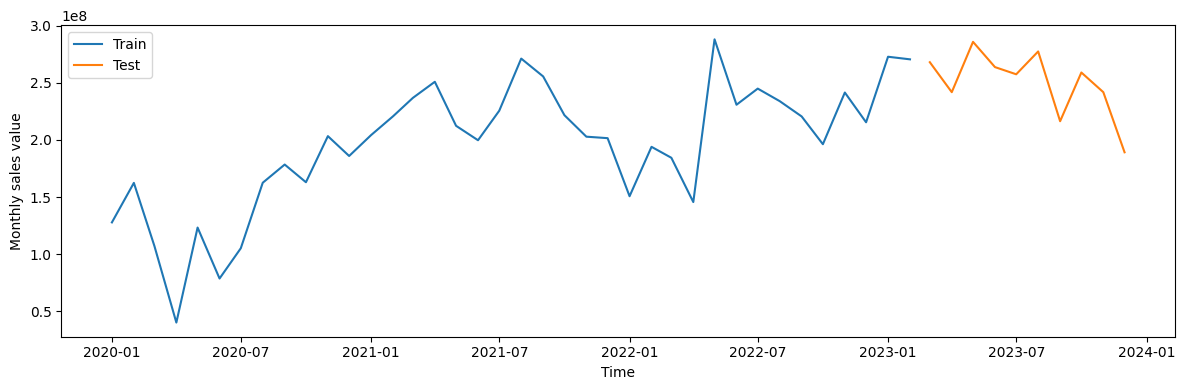
\includegraphics[width=0.94\linewidth]
    {figures/industrial_demand_series.png}
    \caption{Industrial demand series and temporal split.}
    \label{fig:icmd_data_overview}
\end{figure}

Because the anonymized release does not expose the raw product-level industrial
series, the diagnostic values in Table~\ref{tab:icmd_diagnostics} are reported
as audit fields rather than inferred from forecast outputs. They should be
computed directly from the confidential monthly target before final submission;
until then, the interpretation below is restricted to the visible series
profile and benchmark outcomes.

\begin{table}[t]
\centering
\caption{Industrial series diagnostics.}
\label{tab:icmd_diagnostics}
\footnotesize
\setlength{\tabcolsep}{5pt}
\renewcommand{\arraystretch}{0.9999}
\begin{tabular}{|l|c|c|}
\hline
Diagnostic & Raw scale & Log scale \\
\hline
ADF $p$-value & 0.0465 & 0.2910 \\
\hline
KPSS $p$-value & 0.0164 & 0.0217 \\
\hline
Coefficient of variation & 0.2714 & 0.0192 \\
\hline
Lag-1 autocorrelation & 0.7239 & 0.6641 \\
\hline
Lag-12 autocorrelation & 0.0013 & -0.0429 \\
\hline
Seasonal strength & 0.5356 & 0.6310 \\
\hline
Trend strength & 0.8101 & 0.8129 \\
\hline
\end{tabular}
\end{table}

\subsection{Overall Benchmarking and Metric-Specific Behaviour}
\label{subsec:benchmark_results}

Table~\ref{tab:point_performance_vertical} preserves all five datasets and all
model evaluations. Each row represents a dataset--model pair. ICMD
is treated as the primary engineering validation, whereas M4 provides the
principal public and reproducible methodological validation. CIF, M3, and
Tourism are retained to expose both transferability and failure modes.

On ICMD, S3-Forecaster obtains the strongest scale-normalized RMSE and $R^2$,
whereas S3-FastSketch gives the lowest MAPE$_\epsilon$. Chronos is highly
competitive---second in RMSE and $R^2$ and close in MAPE$_\epsilon$---but it
does not dominate all point metrics on the model scale. The
engineering case therefore supports a more nuanced conclusion: a frozen
foundation prior can be strong, but gradient-free residual adaptation remains
competitive and can provide the best variance-sensitive accuracy under an
extremely short industrial history.

On M4, S3-FastSketch obtains the best point-forecasting results across RMSE,
$R^2$, and MAPE$_\epsilon$, while S3-Forecaster is consistently second. This
pattern indicates that the lower-dimensional sketch can be preferable when the
residual structure is sufficiently captured by compact random features. It also
shows that the S3 family benefit is not tied to a single residual representation.

CIF and M3 delimit the method's operating range. On CIF, S3-Forecaster is the
best point model across all three metrics, with S3-FastSketch and Gaussian
Process remaining competitive. On M3, S3-Forecaster and ETS are tied at the best
point values, while Chronos is the strongest non-S3/non-ETS competitor in RMSE
and $R^2$. Tourism provides a complementary case in which S3-FastSketch is best
and EasyTSF is second, showing that compact adaptation may outperform the larger
reservoir when the available history supports a simpler correction. Overall,
Table~\ref{tab:point_performance_vertical} supports selective S3-family
strength rather than universal dominance by a single model.


\begin{table}[p]
\centering
\caption{Point-forecasting results on the model scale.}
\label{tab:point_performance_vertical}
\fontsize{7pt}{7.35pt}\selectfont
\setlength{\tabcolsep}{2.5pt}
\renewcommand{\arraystretch}{0.78}
\begin{tabular}{|>{\centering\arraybackslash}p{1.55cm}|>{\raggedright\arraybackslash}p{2.85cm}|r|r|r|}
\hline
Dataset & Model & RMSE $\downarrow$ & $R^2$ $\uparrow$ & MAPE$_\epsilon$ $\downarrow$ \\
\hline
\multirow{12}{=}{\centering CIF} & S3-Forecaster & \textbf{0.0161} & \textbf{0.5014} & \textbf{0.2103} \\
\cline{2-5}
 & S3-FastSketch & \underline{0.0174} & \underline{0.4163} & 0.2312 \\
\cline{2-5}
 & ARIMA & 0.0251 & -0.2110 & 0.2740 \\
\cline{2-5}
 & AR & 0.0323 & -1.0104 & 0.3908 \\
\cline{2-5}
 & ETS & 0.0225 & 0.0282 & 0.2446 \\
\cline{2-5}
 & Kernel Ridge & 0.0217 & 0.0925 & 0.2569 \\
\cline{2-5}
 & Gaussian Process & 0.0186 & 0.3381 & \underline{0.2179} \\
\cline{2-5}
 & Chronos & 0.0205 & 0.1891 & 0.2303 \\
\cline{2-5}
 & LSTM & 0.0654 & -7.2221 & 0.7513 \\
\cline{2-5}
 & CNN & 0.0319 & -0.9553 & 0.3323 \\
\cline{2-5}
 & AR-KAN & 0.0605 & -6.0433 & 0.7468 \\
\cline{2-5}
 & EasyTSF & 0.0232 & -0.0337 & 0.2550 \\
\hline
\multirow{12}{=}{\centering M3} & S3-Forecaster & \textbf{0.3773} & \textbf{0.0176} & \textbf{3.1504} \\
\cline{2-5}
 & S3-FastSketch & 0.3952 & -0.0777 & \underline{3.2284} \\
\cline{2-5}
 & ARIMA & 0.6076 & -1.5471 & 5.9327 \\
\cline{2-5}
 & AR & 0.4512 & -0.4051 & 3.7083 \\
\cline{2-5}
 & ETS & \textbf{0.3773} & \textbf{0.0176} & \textbf{3.1504} \\
\cline{2-5}
 & Kernel Ridge & 0.7047 & -2.4268 & 7.3793 \\
\cline{2-5}
 & Gaussian Process & 0.5155 & -0.8339 & 5.3484 \\
\cline{2-5}
 & Chronos & \underline{0.3925} & \underline{-0.0631} & 3.2677 \\
\cline{2-5}
 & LSTM & 0.4585 & -0.4508 & 4.2237 \\
\cline{2-5}
 & CNN & 0.4849 & -0.6224 & 4.7572 \\
\cline{2-5}
 & AR-KAN & 0.4272 & -0.2592 & 4.1712 \\
\cline{2-5}
 & EasyTSF & 0.5578 & -1.1466 & 5.7628 \\
\hline
\multirow{12}{=}{\centering ICMD} & S3-Forecaster & \textbf{0.1079} & \textbf{0.1628} & \underline{0.5076} \\
\cline{2-5}
 & S3-FastSketch & 0.1377 & -0.3635 & \textbf{0.4973} \\
\cline{2-5}
 & ARIMA & 19.3307 & -2.689e+04 & 100.0000 \\
\cline{2-5}
 & AR & 0.3145 & -6.1187 & 1.3408 \\
\cline{2-5}
 & ETS & 0.2181 & -2.4226 & 0.8825 \\
\cline{2-5}
 & Kernel Ridge & 0.2650 & -4.0541 & 1.2152 \\
\cline{2-5}
 & Gaussian Process & 0.2517 & -3.5587 & 1.1824 \\
\cline{2-5}
 & Chronos & \underline{0.1122} & \underline{0.0939} & 0.5200 \\
\cline{2-5}
 & LSTM & 0.2552 & -3.6854 & 1.1573 \\
\cline{2-5}
 & CNN & 0.2456 & -3.3413 & 1.1250 \\
\cline{2-5}
 & AR-KAN & 0.1494 & -0.6066 & 0.6820 \\
\cline{2-5}
 & EasyTSF & 0.2096 & -2.1619 & 0.7993 \\
\hline
\multirow{12}{=}{\centering Tourism} & S3-Forecaster & 0.0823 & 0.9636 & 0.8259 \\
\cline{2-5}
 & S3-FastSketch & \textbf{0.0616} & \textbf{0.9795} & \textbf{0.6308} \\
\cline{2-5}
 & ARIMA & 0.1585 & 0.8647 & 1.6908 \\
\cline{2-5}
 & AR & 0.1148 & 0.9290 & 1.1699 \\
\cline{2-5}
 & ETS & 0.0954 & 0.9509 & 0.9212 \\
\cline{2-5}
 & Kernel Ridge & 0.1478 & 0.8824 & 1.5375 \\
\cline{2-5}
 & Gaussian Process & 0.1153 & 0.9284 & 1.1658 \\
\cline{2-5}
 & Chronos & 0.1262 & 0.9143 & 1.3903 \\
\cline{2-5}
 & LSTM & 0.1409 & 0.8930 & 1.4096 \\
\cline{2-5}
 & CNN & 0.1652 & 0.8529 & 1.5454 \\
\cline{2-5}
 & AR-KAN & 0.0948 & 0.9516 & 0.8938 \\
\cline{2-5}
 & EasyTSF & \underline{0.0687} & \underline{0.9746} & \underline{0.6857} \\
\hline
\multirow{12}{=}{\centering M4} & S3-Forecaster & \underline{0.1401} & \underline{0.6866} & \underline{1.3367} \\
\cline{2-5}
 & S3-FastSketch & \textbf{0.1122} & \textbf{0.7990} & \textbf{0.9240} \\
\cline{2-5}
 & ARIMA & 0.2521 & -0.0144 & 2.5713 \\
\cline{2-5}
 & AR & 0.1918 & 0.4129 & 1.6391 \\
\cline{2-5}
 & ETS & 0.1427 & 0.6749 & 1.5010 \\
\cline{2-5}
 & Kernel Ridge & 0.1760 & 0.5055 & 1.6982 \\
\cline{2-5}
 & Gaussian Process & 0.1616 & 0.5832 & 1.6328 \\
\cline{2-5}
 & Chronos & 0.1554 & 0.6149 & 1.5043 \\
\cline{2-5}
 & LSTM & 0.1946 & 0.3956 & 1.9254 \\
\cline{2-5}
 & CNN & 0.1737 & 0.5184 & 1.6041 \\
\cline{2-5}
 & AR-KAN & 0.2560 & -0.0455 & 2.4357 \\
\cline{2-5}
 & EasyTSF & 0.1943 & 0.3977 & 2.0007 \\
\hline
\end{tabular}
\end{table}

Best values are shown in bold and second-best values are underlined within each
dataset and metric.  
\normalsize

% Main-text panels: ICMD demonstrates engineering relevance; M4 demonstrates
% reproducible public-benchmark performance.
% CIF, M3, and Tourism forecast panels can be placed in the supplement.
\begin{figure*}[t]
    \centering
    \begin{subfigure}[t]{0.47\textwidth}
        \centering
        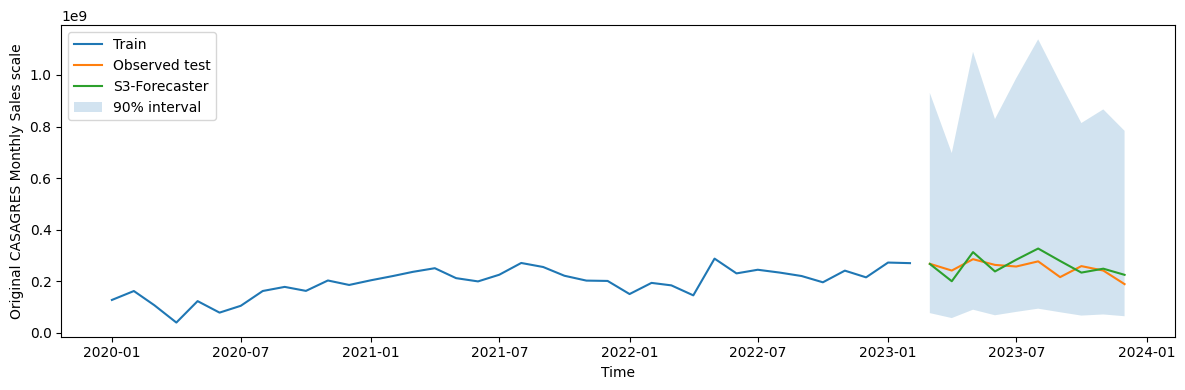
\includegraphics[width=\linewidth]
        {figures/industrial_demand_s3_forecast.png}
        \caption{ICMD}
    \end{subfigure}
    \hfill
    \begin{subfigure}[t]{0.47\textwidth}
        \centering
        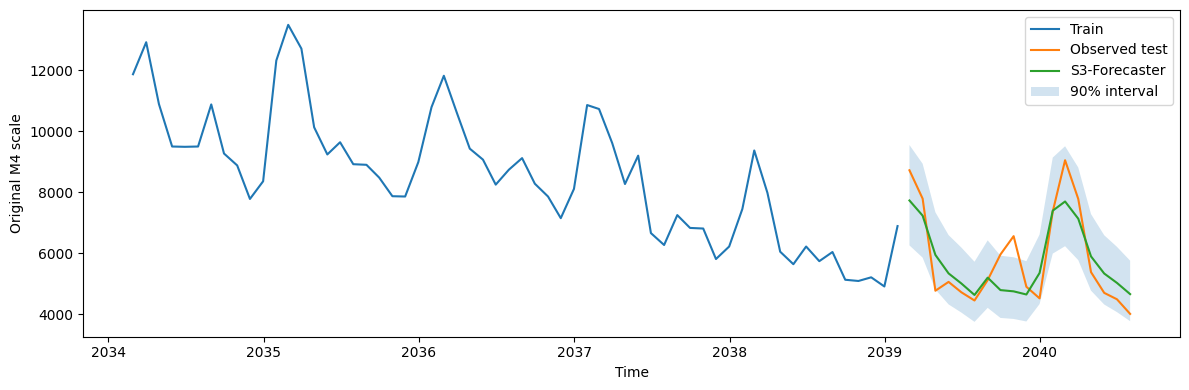
\includegraphics[width=\linewidth]
        {figures/m4_s3_forecast.png}
        \caption{M4}
    \end{subfigure}
    \caption{Primary test forecasts.}
    \label{fig:primary_forecasts}
\end{figure*}

\subsection{Component-Wise Ablation Study}
\label{subsec:ablation_results}

Table~\ref{tab:s3_ablation_vertical} separates the frozen causal prior, the
ESN-based residual adapter, the OOB volatility gate, and the adaptive conformal
uncertainty layer. The residual adapter has conditional rather than uniform
utility. Let $e_t$ denote the base residual and $\widehat r_t$ the adapter
correction. For a gate value $g_t$, the change in expected squared error is
\begin{equation}
\mathbb{E}\!\left[(e_t-g_t\widehat r_t)^2-e_t^2\right]
=
\mathbb{E}[g_t^2\widehat r_t^2]
-
2\mathbb{E}[g_te_t\widehat r_t].
\label{eq:residual_correction_utility}
\end{equation}
A correction is useful only when its alignment with the future base residual
is sufficiently large to offset the variance introduced by the correction
itself. This condition is difficult to estimate reliably when $N<200$, even
when the readout is obtained through a stable convex regularized objective.

M4 provides the clearest adapter contribution: MAPE$_\epsilon$ decreases from
$1.5576$ for the frozen prior to $1.3367$ after residual adaptation, a relative
reduction of approximately $14.2\%$. The gate remains equal to one, indicating
that the improvement is driven by the residual representation and readout
rather than by attenuation.

ICMD exhibits the complementary mechanism. The ungated adapter produces only a
small MAPE degradation relative to the prior, but the OOB gate reduces MAPE
from $0.6758$ to $0.6246$ and RMSE from $0.1465$ to $0.1403$, with a mean gate
of $0.662$. Hence, the gate provides its most substantive marginal contribution
in the engineering case by suppressing over-correction. On M3, Tourism, and M4,
the mean gate remains between $0.971$ and $1.000$ and therefore behaves
approximately as an identity mapping.

CIF is an explicit negative-transfer case: the adapter increases error and the
gate recovers only part of the loss. This result supports interpreting the gate
as a protective shrinkage mechanism rather than a component that guarantees
independent improvement.

\begin{table}[!htbp]
\centering
\caption{Component-wise ablation results for S3-Forecaster. Point metrics are unchanged by the uncertainty layer; ECP and MSIS are reported only for conformal variants.}
\label{tab:s3_ablation_vertical}
\scriptsize
\setlength{\tabcolsep}{3pt}
\renewcommand{\arraystretch}{0.9999}
\begin{tabular}{|>{\centering\arraybackslash}p{1.45cm}|l|r|r|r|r|r|}
\hline
Dataset & Variant & MAPE$_\epsilon$ $\downarrow$ & RMSE $\downarrow$ & Mean gate & ECP & MSIS $\downarrow$ \\
\hline
\multirow{5}{=}{\centering CIF} & Base only & \textbf{0.3669} & \textbf{0.0310} & -- & -- & -- \\
\cline{2-7}
 & Base + residual adapter & 0.5536 & 0.0460 & 1.000 & -- & -- \\
\cline{2-7}
 & Base + residual + gate & \underline{0.4449} & \underline{0.0385} & 0.870 & -- & -- \\
\cline{2-7}
 & Full model + ACI & 0.4449 & 0.0385 & 0.870 & 1.000 & 2.8417 \\
\cline{2-7}
 & Full model + static conformal & 0.4449 & 0.0385 & 0.870 & 0.750 & \textbf{2.0647} \\
\hline
\multirow{5}{=}{\centering M3} & Base only & \textbf{3.4204} & \textbf{0.4324} & -- & -- & -- \\
\cline{2-7}
 & Base + residual adapter & 3.7051 & 0.4716 & 1.000 & -- & -- \\
\cline{2-7}
 & Base + residual + gate & \underline{3.7042} & \underline{0.4715} & 0.998 & -- & -- \\
\cline{2-7}
 & Full model + ACI & 3.7042 & 0.4715 & 0.998 & 0.611 & 5.7616 \\
\cline{2-7}
 & Full model + static conformal & 3.7042 & 0.4715 & 0.998 & 0.611 & \textbf{5.7608} \\
\hline
\multirow{5}{=}{\centering ICMD} & Base only & \underline{0.6708} & 0.1593 & -- & -- & -- \\
\cline{2-7}
 & Base + residual adapter & 0.6758 & \underline{0.1465} & 1.000 & -- & -- \\
\cline{2-7}
 & Base + residual + gate & \textbf{0.6246} & \textbf{0.1403} & 0.662 & -- & -- \\
\cline{2-7}
 & Full model + ACI & 0.6246 & 0.1403 & 0.662 & 0.900 & \textbf{1.2908} \\
\cline{2-7}
 & Full model + static conformal & 0.6246 & 0.1403 & 0.662 & 0.900 & \textbf{1.2908} \\
\hline
\multirow{5}{=}{\centering Tourism} & Base only & \textbf{0.7179} & \textbf{0.0681} & -- & -- & -- \\
\cline{2-7}
 & Base + residual adapter & 0.8306 & 0.0828 & 1.000 & -- & -- \\
\cline{2-7}
 & Base + residual + gate & \underline{0.8259} & \underline{0.0823} & 0.971 & -- & -- \\
\cline{2-7}
 & Full model + ACI & 0.8259 & 0.0823 & 0.971 & 1.000 & \textbf{12.5348} \\
\cline{2-7}
 & Full model + static conformal & 0.8259 & 0.0823 & 0.971 & 1.000 & 17.6732 \\
\hline
\multirow{5}{=}{\centering M4} & Base only & 1.5576 & 0.1509 & -- & -- & -- \\
\cline{2-7}
 & Base + residual adapter & \textbf{1.3367} & \textbf{0.1401} & 1.000 & -- & -- \\
\cline{2-7}
 & Base + residual + gate & \textbf{1.3367} & \textbf{0.1401} & 1.000 & -- & -- \\
\cline{2-7}
 & Full model + ACI & 1.3367 & 0.1401 & 1.000 & 1.000 & 6.9809 \\
\cline{2-7}
 & Full model + static conformal & 1.3367 & 0.1401 & 1.000 & 0.944 & \textbf{4.8546} \\
\hline
\end{tabular}
\end{table}

% Main-text panels: ICMD highlights the gate; M4 highlights the adapter.
% The remaining dataset panels can be included in supplementary material.
\begin{figure*}[t]
    \centering
    \begin{subfigure}[t]{0.47\textwidth}
        \centering
        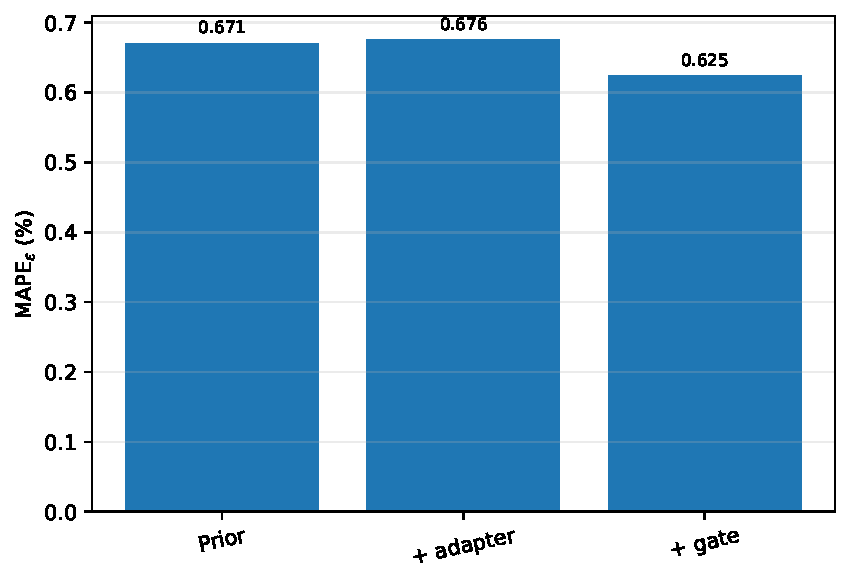
\includegraphics[width=\linewidth]
        {figures/ablation_icmd.pdf}
        \caption{ICMD}
    \end{subfigure}
    \hfill
    \begin{subfigure}[t]{0.47\textwidth}
        \centering
        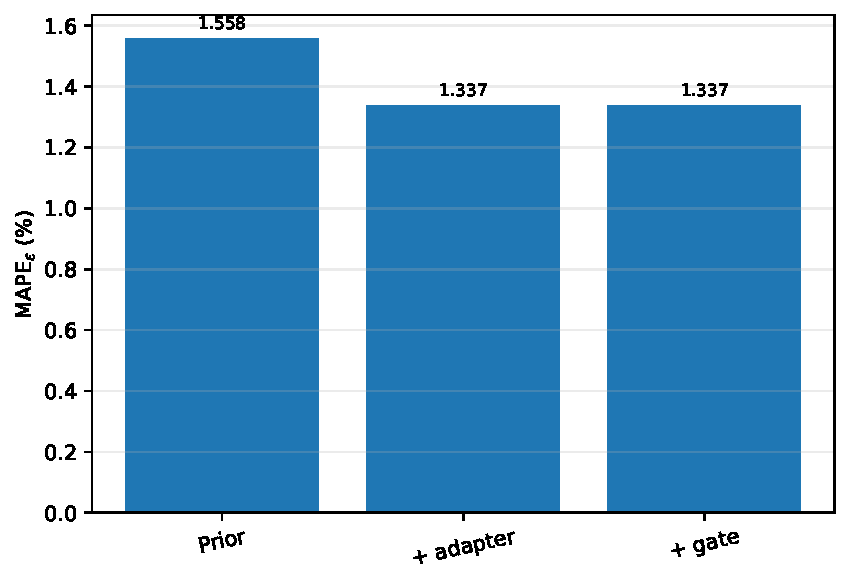
\includegraphics[width=\linewidth]
        {figures/ablation_m4.pdf}
        \caption{M4}
    \end{subfigure}
    \caption{Component-wise ablation for the S3-Forecaster.}
    \label{fig:primary_ablation}
\end{figure*}

\subsection{Adaptive Conformal Uncertainty Estimation}
\label{subsec:adaptive_conformal_results}

Table~\ref{tab:uq_performance_vertical} combines adaptive conformal uncertainty metrics with operational runtime and trainable-parameter counts for the same dataset--model rows. In the uncertainty columns, ECP is interpreted through its absolute deviation from the nominal level $0.90$, while MSIS remains the principal joint criterion because it penalizes both width and misses.
% \begin{equation}
% \mathrm{IS}_{\delta,t}
% =
% (U_t-L_t)
% +
% \frac{2}{\delta}(L_t-y_t)\mathbb{I}\{y_t<L_t\}
% +
% \frac{2}{\delta}(y_t-U_t)\mathbb{I}\{y_t>U_t\}.
% \end{equation}
Consequently, coverage above the nominal level is not intrinsically preferable
when it is achieved through excessive width.

On M4, S3-Forecaster obtains the lowest MSIS ($4.6380$), but its ECP is
$0.833$. The result supports efficient adaptive conformal uncertainty
estimation, not exact nominal coverage on a short test block. S3-FastSketch is
second under MSIS on M4, which mirrors its strong point-forecasting performance
but with slightly less favorable interval quality.

On ICMD, Chronos obtains the lowest MSIS ($1.3580$) with zero target-trainable
parameters, while S3-Forecaster reaches ECP=$1.0$ but produces the largest MSIS,
revealing over-conservative intervals on the model scale. Thus, the best
point-forecasting behavior of S3-Forecaster on ICMD does not automatically
transfer to interval efficiency.

M3 remains the clearest uncertainty limitation for S3-Forecaster: its ECP is
$0.611$, indicating that the calibration residuals are not representative of
the subsequent test errors. LSTM and CNN obtain the strongest MSIS values on M3,
whereas Chronos achieves high empirical coverage with wider intervals. CIF
favors S3-Forecaster under MSIS, while Tourism favors S3-FastSketch and places
Chronos behind ETS under the interval-score criterion. These results show that
adaptive conformal estimation remains sensitive to both calibration
representativeness and the point-forecast residual geometry.

Because the test blocks contain only 10--24 observations, empirical coverage is
highly discrete. If $k$ observations are covered in a test block of size $T$,
% \begin{equation}
%     \widehat{\mathrm{ECP}}=\frac{k}{T},
% \end{equation}
and one additional miss changes ECP by $1/T$. The observed ECP values should
therefore not be interpreted as exact finite-sample
distribution-free predictive validity. The conformal construction avoids a
parametric residual law, but its practical short-block validity depends on the
sequential calibration conditions and on the evolution of the nonconformity
scores.



\begin{table}[p]
\centering
\caption{Adaptive conformal uncertainty and operational-efficiency results on the model scale.}
\label{tab:uq_performance_vertical}
\label{tab:efficiency_vertical}
\scriptsize
\setlength{\tabcolsep}{1.5pt}
\renewcommand{\arraystretch}{0.52}
\begin{tabular}{|>{\centering\arraybackslash}p{1.15cm}|>{\raggedright\arraybackslash}p{2.25cm}|r|r|r|r|r|}
\hline
Dataset & Model & ECP $\rightarrow 0.90$ & IW & MSIS $\downarrow$ & Time (s) $\downarrow$ & Params $\downarrow$ \\
\hline
\multirow{12}{=}{\centering CIF} & S3-Forecaster & 1.000 & 0.1098 & \textbf{1.4965} & 0.8168 & 554 \\
\cline{2-7}
 & S3-FastSketch & 1.000 & 0.1549 & 2.1119 & 1.7267 & 24 \\
\cline{2-7}
 & ARIMA & 1.000 & 0.1674 & 2.2810 & 0.3818 & 7 \\
\cline{2-7}
 & AR & \textbf{0.917} & 0.1658 & 2.2648 & \underline{0.0078} & \underline{2} \\
\cline{2-7}
 & ETS & 1.000 & 0.1959 & 2.6706 & 0.1134 & 18 \\
\cline{2-7}
 & Kernel Ridge & 1.000 & 0.2006 & 2.7341 & \textbf{0.0043} & 792 \\
\cline{2-7}
 & Gaussian Process & 1.000 & 0.2763 & 3.7665 & 0.5911 & 1,032 \\
\cline{2-7}
 & Chronos & 1.000 & 0.1524 & 2.0767 & 2.2445 & \textbf{0} \\
\cline{2-7}
 & LSTM & \underline{0.833} & 0.2080 & 3.4810 & 4.6291 & 10,124 \\
\cline{2-7}
 & CNN & 1.000 & 0.4208 & 5.7350 & 5.1261 & 65,372 \\
\cline{2-7}
 & AR-KAN & 1.000 & 0.3996 & 5.4469 & 2.5985 & 199,975 \\
\cline{2-7}
 & EasyTSF & 1.000 & 0.1372 & \underline{1.8696} & 1.5703 & 5 \\
\hline
\multirow{12}{=}{\centering M3} & S3-Forecaster & 0.611 & 0.4658 & 4.3695 & 0.5483 & 1,082 \\
\cline{2-7}
 & S3-FastSketch & \textbf{0.944} & 1.5346 & 4.0887 & 3.7622 & 32 \\
\cline{2-7}
 & ARIMA & \textbf{0.944} & 2.3480 & 5.8136 & 0.1613 & 5 \\
\cline{2-7}
 & AR & \textbf{0.944} & 2.2877 & 5.2701 & \underline{0.0109} & \underline{3} \\
\cline{2-7}
 & ETS & \textbf{0.944} & 2.1689 & 4.2279 & 0.1692 & 18 \\
\cline{2-7}
 & Kernel Ridge & \textbf{0.944} & 2.2639 & 4.4071 & \textbf{0.0047} & 414 \\
\cline{2-7}
 & Gaussian Process & \underline{1.000} & 1.9709 & 3.4225 & 0.6895 & 468 \\
\cline{2-7}
 & Chronos & \textbf{0.944} & 2.1647 & 4.1557 & 1.3550 & \textbf{0} \\
\cline{2-7}
 & LSTM & \underline{1.000} & 1.8993 & \textbf{3.2980} & 16.0110 & 90,450 \\
\cline{2-7}
 & CNN & \underline{1.000} & 1.9435 & \underline{3.3747} & 4.0094 & 11,978 \\
\cline{2-7}
 & AR-KAN & \textbf{0.944} & 2.0599 & 3.6728 & 3.8750 & 79,116 \\
\cline{2-7}
 & EasyTSF & \textbf{0.944} & 2.1698 & 4.0885 & 0.3185 & \underline{3} \\
\hline
\multirow{12}{=}{\centering ICMD} & S3-Forecaster & \underline{1.000} & 4.3752 & 11.1116 & 2.3646 & 802 \\
\cline{2-7}
 & S3-FastSketch & \textbf{0.900} & 0.4078 & 1.7512 & 9.5540 & 29 \\
\cline{2-7}
 & ARIMA & \textbf{0.900} & 38.9134 & 99.0639 & 0.0158 & \underline{1} \\
\cline{2-7}
 & AR & \underline{1.000} & 1.2365 & 3.1403 & \underline{0.0084} & 15 \\
\cline{2-7}
 & ETS & \underline{1.000} & 0.9636 & 2.4471 & 0.1062 & 18 \\
\cline{2-7}
 & Kernel Ridge & \underline{1.000} & 0.9650 & 2.4507 & \textbf{0.0045} & 270 \\
\cline{2-7}
 & Gaussian Process & \textbf{0.900} & 0.7567 & 2.3255 & 0.5511 & 270 \\
\cline{2-7}
 & Chronos & \underline{1.000} & 0.5347 & \textbf{1.3580} & 1.0396 & \textbf{0} \\
\cline{2-7}
 & LSTM & \underline{1.000} & 0.8215 & 2.0863 & 9.9215 & 284,228 \\
\cline{2-7}
 & CNN & \underline{1.000} & 0.8407 & 2.1351 & 3.7897 & 23,194 \\
\cline{2-7}
 & AR-KAN & \underline{1.000} & 0.6425 & \underline{1.6317} & 1.1184 & 18,840 \\
\cline{2-7}
 & EasyTSF & \underline{0.800} & 0.5618 & 2.5675 & 0.1806 & 5 \\
\hline
\multirow{12}{=}{\centering Tourism} & S3-Forecaster & 1.000 & 0.8064 & 10.1517 & 0.0761 & 842 \\
\cline{2-7}
 & S3-FastSketch & 0.792 & 0.1395 & \textbf{3.8261} & 4.1925 & 27 \\
\cline{2-7}
 & ARIMA & 0.958 & 0.6655 & 8.3783 & 1.0799 & \underline{13} \\
\cline{2-7}
 & AR & \textbf{0.917} & 0.4346 & 6.0169 & \underline{0.0127} & 28 \\
\cline{2-7}
 & ETS & 0.792 & 0.3014 & \underline{4.7576} & 0.1461 & 18 \\
\cline{2-7}
 & Kernel Ridge & 0.750 & 0.3449 & 6.6261 & \textbf{0.0057} & 2,376 \\
\cline{2-7}
 & Gaussian Process & 1.000 & 0.8237 & 10.3698 & 4.6365 & 3,000 \\
\cline{2-7}
 & Chronos & \textbf{0.917} & 0.4287 & 5.6795 & 1.0096 & \textbf{0} \\
\cline{2-7}
 & LSTM & \underline{0.875} & 0.4954 & 7.7034 & 11.7454 & 28,312 \\
\cline{2-7}
 & CNN & \textbf{0.917} & 0.6913 & 9.9082 & 12.3743 & 2,192 \\
\cline{2-7}
 & AR-KAN & 1.000 & 0.6234 & 7.8473 & 2.8422 & 219,483 \\
\cline{2-7}
 & EasyTSF & 1.000 & 0.4164 & 5.2420 & 1.5747 & 20 \\
\hline
\multirow{12}{=}{\centering M4} & S3-Forecaster & \textbf{0.833} & 0.4227 & \textbf{4.6380} & \underline{0.0823} & 182 \\
\cline{2-7}
 & S3-FastSketch & 0.778 & 0.2964 & \underline{4.7737} & 0.9148 & 27 \\
\cline{2-7}
 & ARIMA & \underline{1.000} & 1.1254 & 9.2515 & 1.9694 & \underline{10} \\
\cline{2-7}
 & AR & \underline{1.000} & 1.7706 & 14.5559 & \textbf{0.0337} & 47 \\
\cline{2-7}
 & ETS & \underline{1.000} & 1.3009 & 10.6950 & 0.1534 & 18 \\
\cline{2-7}
 & Kernel Ridge & \underline{1.000} & 1.0498 & 8.6304 & 0.1398 & 7,542 \\
\cline{2-7}
 & Gaussian Process & \underline{1.000} & 1.2014 & 9.8763 & 32.7088 & 7,848 \\
\cline{2-7}
 & Chronos & \underline{1.000} & 1.1137 & 9.1554 & 1.4109 & \textbf{0} \\
\cline{2-7}
 & LSTM & \underline{1.000} & 1.1817 & 9.7147 & 12.6594 & 6,002 \\
\cline{2-7}
 & CNN & \underline{1.000} & 1.1869 & 9.7574 & 9.0094 & 42,306 \\
\cline{2-7}
 & AR-KAN & \underline{1.000} & 1.4715 & 12.0972 & 6.0473 & 3,312 \\
\cline{2-7}
 & EasyTSF & \underline{1.000} & 1.4474 & 11.8990 & 0.9907 & 25 \\
\hline
\end{tabular}
\end{table}



Note that for ECP, bold and underlined entries denote the smallest and second-smallest
absolute deviations from $0.90$. For MSIS, runtime, and trainable parameters,
lower is better. Interval width is reported descriptively. Time measures the
operational fit-and-forecast stage after offline HPO; parameter counts exclude
fixed reservoir matrices and frozen prior parameters. A one-observation change
modifies ECP by $0.10$ on ICMD, $0.083$ on CIF, $0.056$ on M3 and M4, and
$0.042$ on Tourism.
\normalsize

% \subsection{Non-Stationary Regime Diagnostics}
% \label{subsec:nonstationary_regimes}

The causal volatility indicator was retained as a diagnostic of local
distributional change. However, no test observation exceeded the fixed
pre-test threshold in any dataset, as reported in
Table~\ref{tab:volatility_diagnostics}. Overall metrics therefore coincide with
the metrics of the regular test regime, and no separate extreme-regime
performance estimate is available.

% This outcome changes the scope of the empirical claim. The experiments support
% forecasting under short and non-stationary histories, but they do not establish
% performance during threshold-defined discontinuities. The gate can still vary
% continuously below the threshold, as observed on ICMD, but its effect should be
% interpreted as volatility-responsive correction control rather than as evidence
% of recovery from an abrupt event.

\begin{table}[t]
\centering
\caption{Causal volatility diagnostics.}
\label{tab:volatility_diagnostics}
\footnotesize
\setlength{\tabcolsep}{5pt}
\renewcommand{\arraystretch}{0.9999}
\begin{tabular}{|c|r|r|r|r|}
\hline
Dataset & Test size & Threshold $\tau$ & Maximum indicator & Exceedances \\
\hline
CIF     & 12 & 0.1624 & 0.0953 & 0 \\
\hline
M3      & 18 & 1.5929 & 1.1934 & 0 \\
\hline
ICMD    & 10 & 1.1210 & 0.5069 & 0 \\
\hline
Tourism & 24 & 0.2398 & 0.1851 & 0 \\
\hline
M4      & 18 & 0.3596 & 0.2760 & 0 \\
\hline
\end{tabular}
\end{table}

% Each panel displays the causal test indicator and its threshold.
% No event annotation is required because all indicators remain below tau.
\begin{figure*}[t]
    \centering
    \begin{subfigure}[t]{0.47\textwidth}
        \centering
        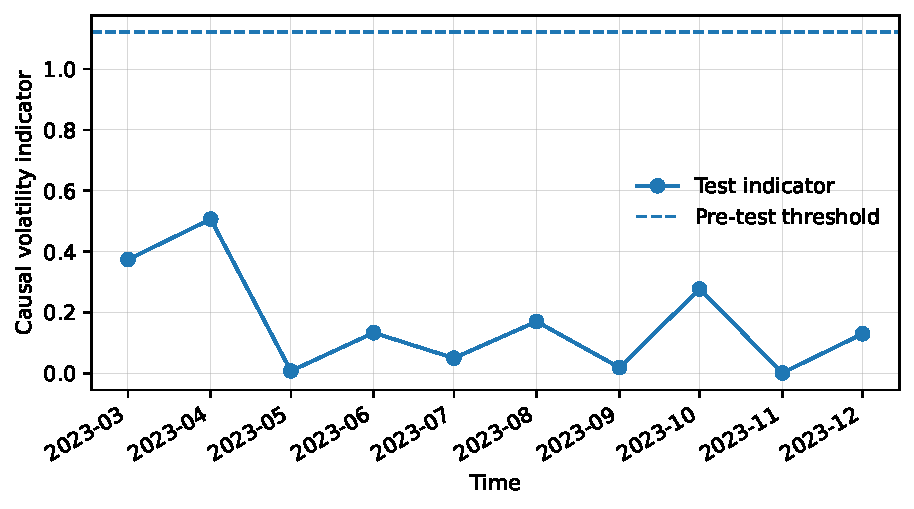
\includegraphics[width=\linewidth]
        {figures/industrial_demand_volatility.pdf}
        \caption{ICMD}
    \end{subfigure}
    \hfill
    \begin{subfigure}[t]{0.47\textwidth}
        \centering
        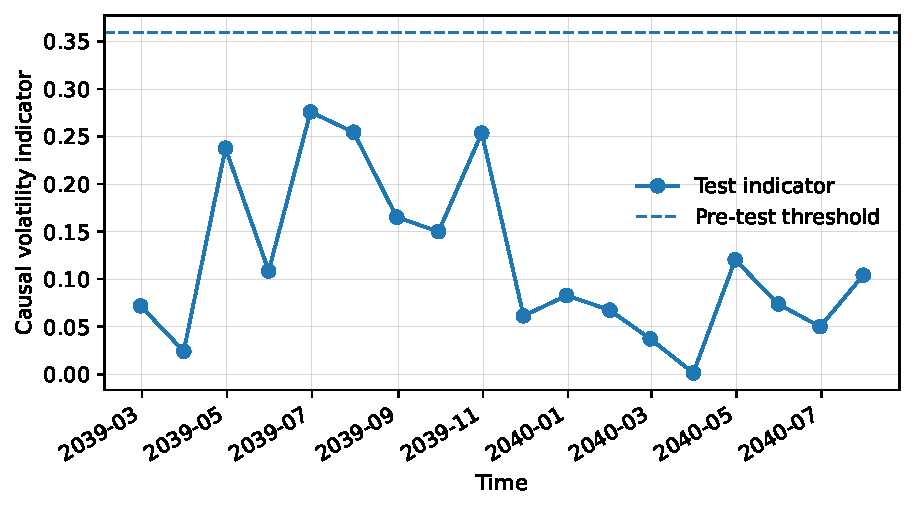
\includegraphics[width=\linewidth]
        {figures/m4_volatility.pdf}
        \caption{M4}
    \end{subfigure}
    \caption{Causal volatility diagnostics.}
    \label{fig:volatility_diagnostics}
\end{figure*}

\subsection{Data Efficiency and History-Length Spectrum}
\label{subsec:data_efficiency_results}

The reduced-history experiments identify a dataset-dependent operating regime.
The panels report MAPE in percentage units as a function of the
available history length, so they should be read as trajectory-level evidence
rather than as a duplicate of the single split in
Table~\ref{tab:point_performance_vertical}.

Across ICMD and M4, the S3 family occupies the most favorable region of the
curves over substantial portions of the history spectrum. This is consistent
with the benchmark table: S3-Forecaster is strongest on ICMD for
variance-sensitive point accuracy, whereas S3-FastSketch is strongest on M4 and
also competitive in ICMD proportional error. The profiles also show that adding
observations is not automatically beneficial; gains appear when the additional
history is relevant to the current regime and when the residual representation
has enough support to estimate a stable readout.

Tourism exhibits a crossover pattern rather than a single dominant curve.
S3-FastSketch, S3-Forecaster, EasyTSF, and ETS exchange relative positions as
history length changes, which is compatible with an approximation--estimation
trade-off. Compact residual features can control variance at shorter or
intermediate histories, while more conventional or trained alternatives can
become competitive once their parameters are sufficiently identified.

CIF and M3 again expose limitations. CIF shows that the S3 family can be strong
on the final split while still exhibiting sensitivity to which historical window
is available. M3 spans a narrow history range and does not provide enough
variation to infer a stable data-efficiency crossover. A useful conceptual
quantity is therefore the effective history size
\begin{equation}
N_{\mathrm{eff}}
=
\frac{\left(\sum_{t=1}^{N}w_t\right)^2}
{\sum_{t=1}^{N}w_t^2},
\end{equation}
where $w_t$ denotes the relevance of observation $t$ to the current regime.
The results indicate that S3-family models benefit from additional data only
when the added observations increase $N_{\mathrm{eff}}$, not merely nominal $N$.

% Five panels, one per dataset. Each panel contains MAPE_epsilon against
% available history for all successful methods. Do not plot failed runs.
\begin{figure*}[t]
    \centering
    \begin{subfigure}[t]{0.32\textwidth}
        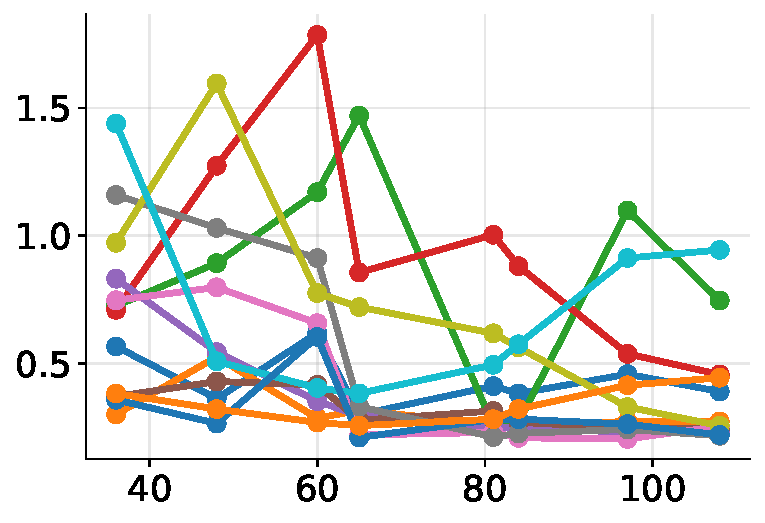
\includegraphics[width=\linewidth]
        {figures/cif_data_efficiency_mape_percent.pdf}
        \caption{CIF}
    \end{subfigure}\hfill
    \begin{subfigure}[t]{0.32\textwidth}
        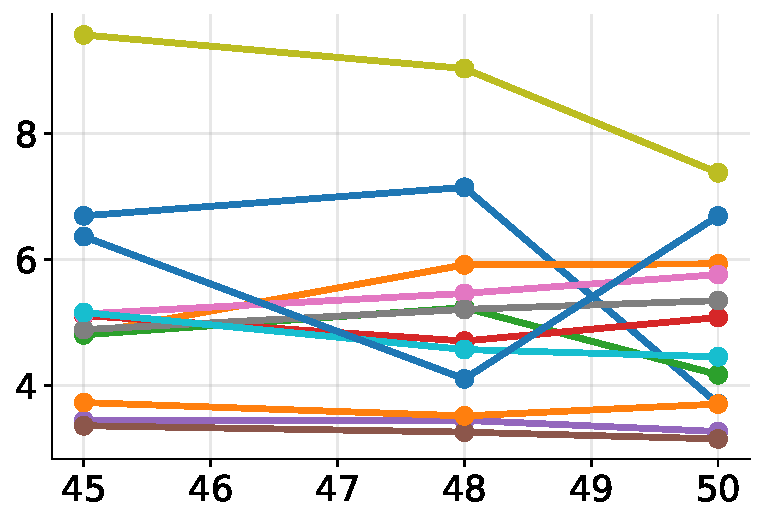
\includegraphics[width=\linewidth]
        {figures/m3_data_efficiency_mape_percent.pdf}
        \caption{M3}
    \end{subfigure}\hfill
    \begin{subfigure}[t]{0.32\textwidth}
        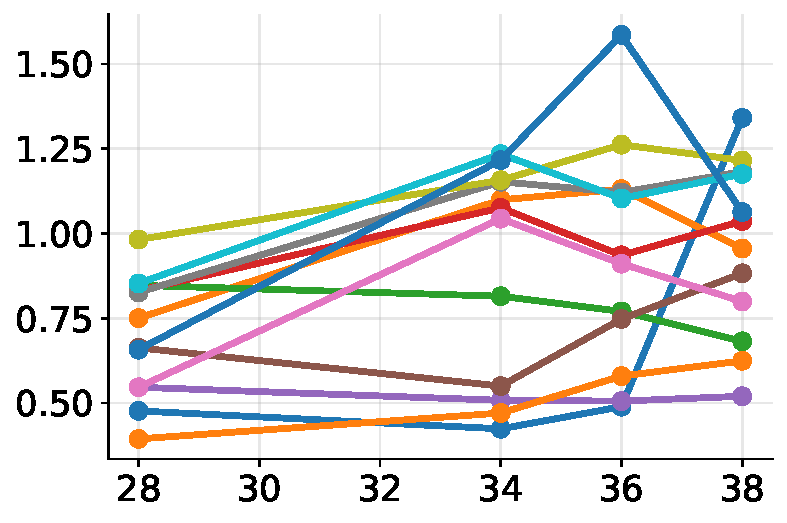
\includegraphics[width=\linewidth]
        {figures/ICMD_Dataset_data_efficiency_mape_percent.pdf}
        \caption{ICMD}
    \end{subfigure}

    \medskip
    \begin{subfigure}[t]{0.32\textwidth}
        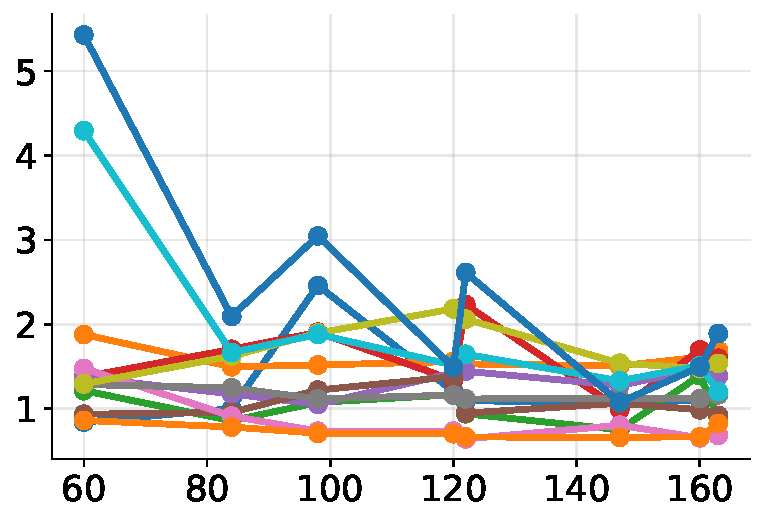
\includegraphics[width=\linewidth]
        {figures/tourism_data_efficiency_mape_percent.pdf}
        \caption{Tourism}
    \end{subfigure}\hfill
    \begin{subfigure}[t]{0.32\textwidth}
        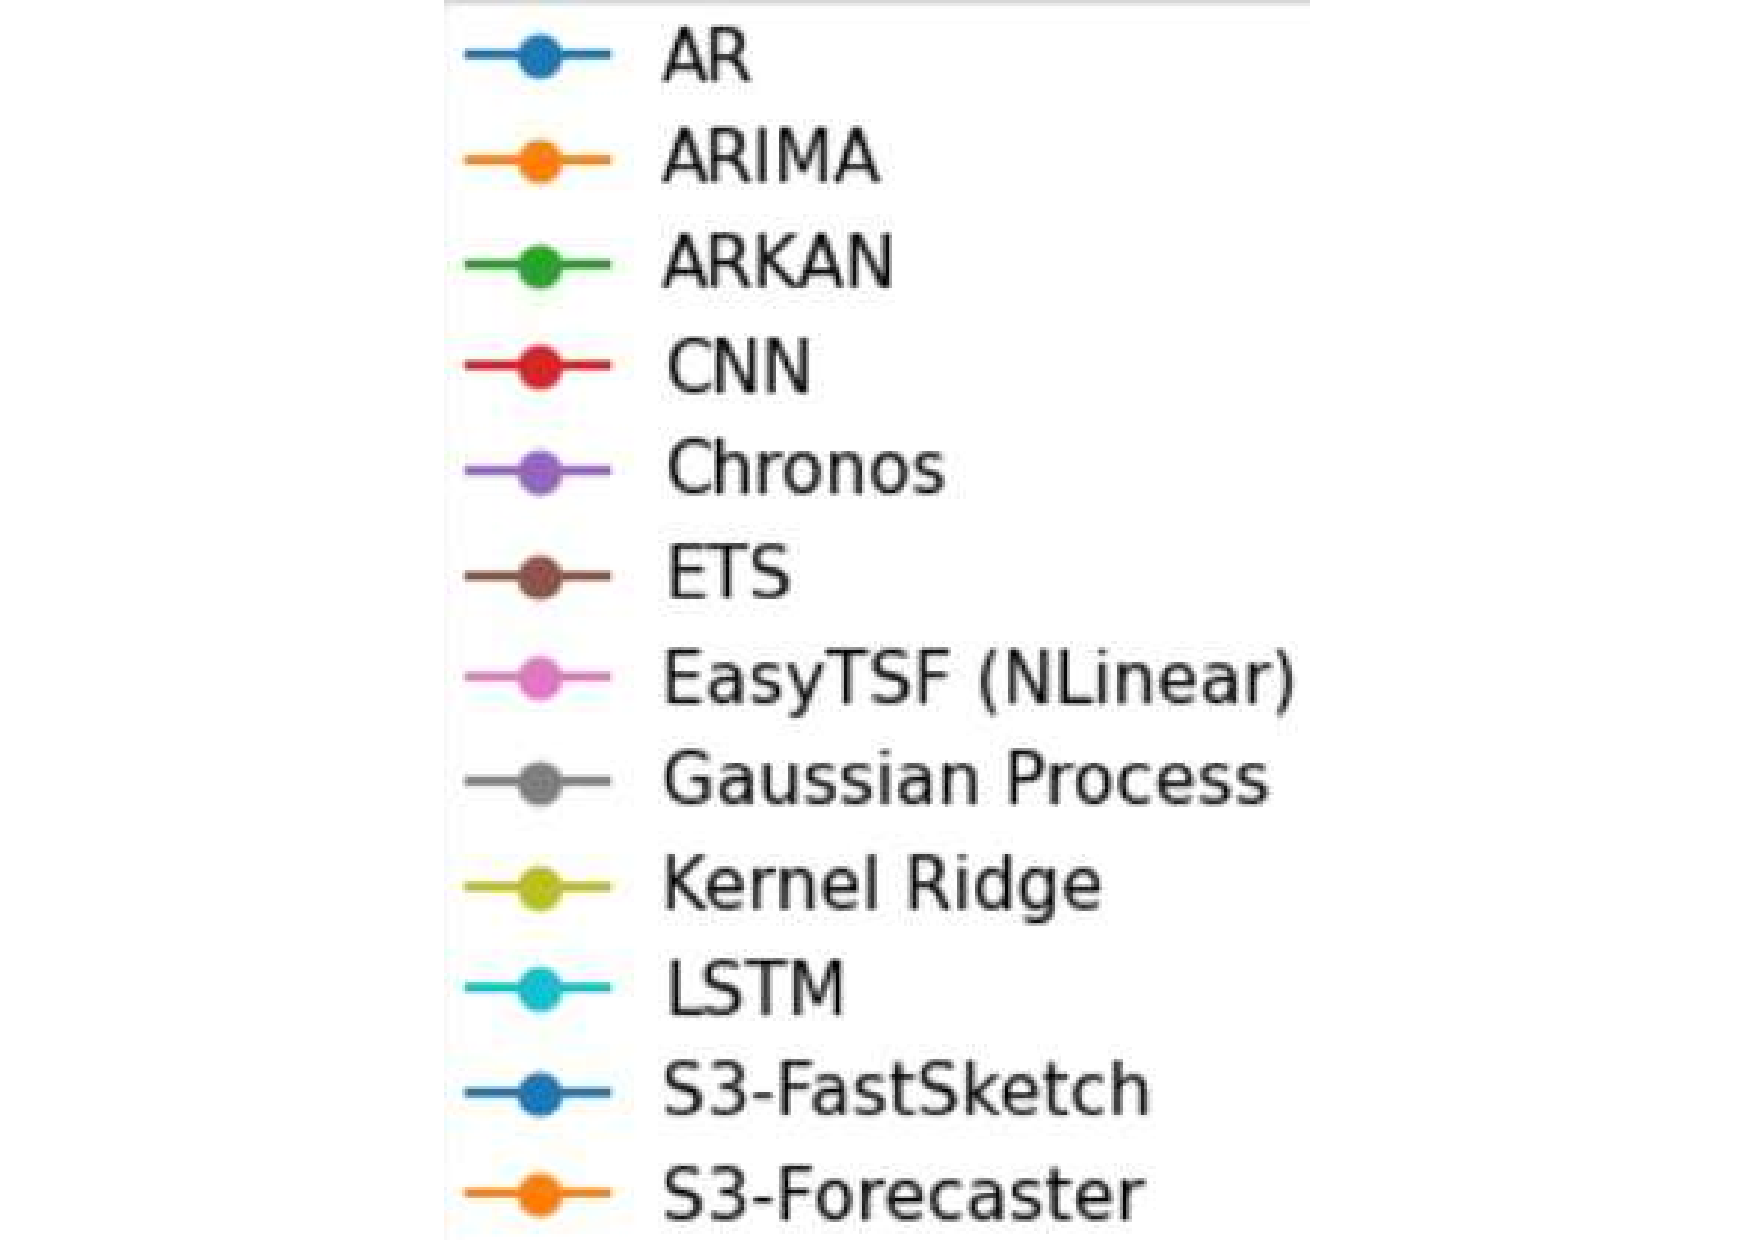
\includegraphics[width=\linewidth]
        {figures/modelos.pdf}
        \caption{Model colors}
    \end{subfigure}\hfill
    \begin{subfigure}[t]{0.32\textwidth}
        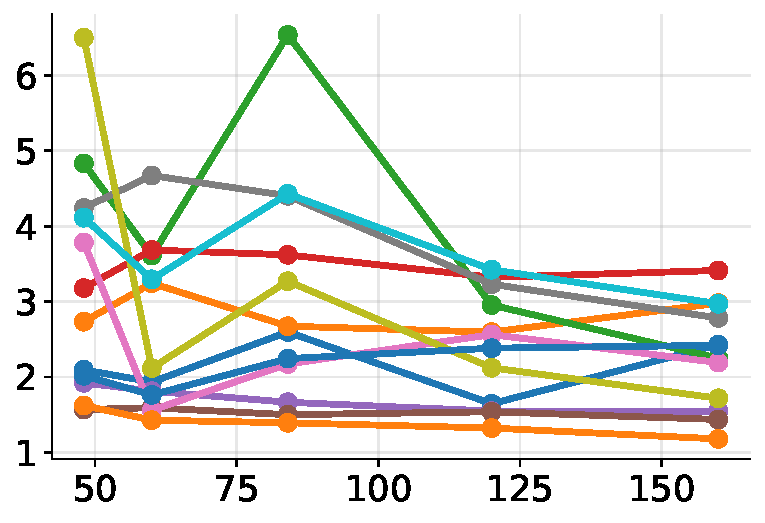
\includegraphics[width=\linewidth]
        {figures/M4_data_efficiency_mape_percent.pdf}
        \caption{M4}
    \end{subfigure}
    \caption{Data-efficiency profiles. The horizontal axis shows the available history and the vertical axis reports MAPE as a percentage.}
    \label{fig:data_efficiency_all_datasets}
\end{figure*}

\subsection{Multi-Prior Robustness and Backbone Transferability}
\label{subsec:multiprior_results}

The prior-transfer experiment evaluates Rolling, ETS, and Prophet backbones.
The multi-prior panels reinforce architectural compatibility, but they
also make clear that performance is not backbone invariant. Across datasets,
residual adaptation is useful only when the chosen prior leaves a stable and
causally predictable residual component. When the prior already captures the
main dynamics, or when its residuals change regime across train, calibration,
and test, the adapter can add variance rather than reduce error.

The qualitative pattern is consistent with the benchmark and data-efficiency
figures. ICMD and M4 provide the strongest evidence that an S3 correction can be
useful under favorable residual structure, but CIF, M3, and Tourism show that
changing the backbone can reverse the ordering among S3-Forecaster,
S3-FastSketch, and the prior-only alternatives. The model-color panel in
Figure~\ref{fig:multi_prior_all_datasets} should therefore be read as a map of
backbone sensitivity rather than as evidence for a universally transferable
adapter.

Let the prior residual admit the decomposition
\begin{equation}
e_t
=
m(\mathbf{h}_{t-1})+\xi_t,
\end{equation}
where $m(\mathbf{h}_{t-1})$ is the component predictable from the causal state
and $\xi_t$ is an innovation. The potential value of residual adaptation is
governed by
\begin{equation}
\operatorname{Var}
\left[
\mathbb{E}
\left(
e_t\mid\mathbf{h}_{t-1}
\right)
\right].
\end{equation}
When this quantity is small, the adapter mainly adds estimation variance.
When it is large and stable across train, calibration, and test, the adapter can
correct systematic prior mismatch.

A severe mismatch exceeds the ESN's corrective capacity when the residual
trajectory lies outside the calibration support, changes sign across regimes,
or contains temporal structure absent from the fixed reservoir state space.
Neither the gate nor the convex readout can reconstruct information that is not
represented in the causal features. This explains why architectural
transferability should not be interpreted as backbone-independent accuracy.

Although Chronos is included in the direct benchmark, the prior-transfer
experiment does not include Chronos as a backbone within the S3 adaptation
pipeline. Accordingly, the prior-transfer results should not be interpreted as a
direct test of foundation-model residual mismatch.

% Five panels, one per dataset. Each panel compares prior-only,
% S3-Forecaster, and S3-FastSketch under Rolling, ETS, and Prophet.
\begin{figure*}[t]
    \centering
    \begin{subfigure}[t]{0.32\textwidth}
        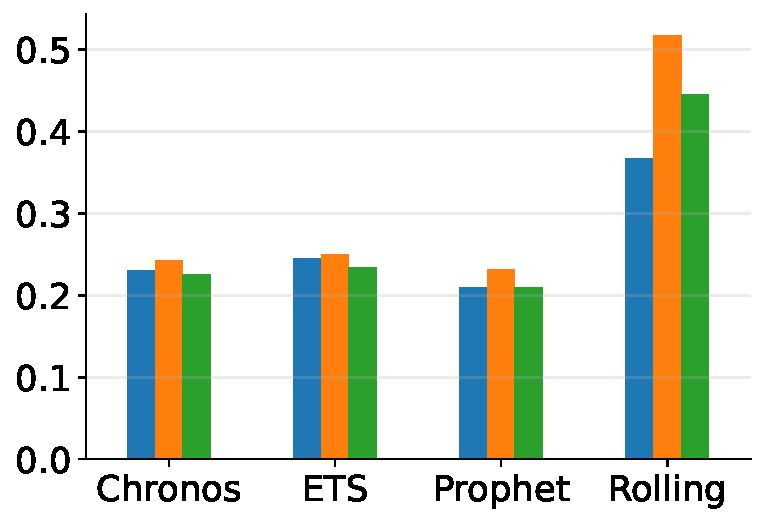
\includegraphics[width=\linewidth]
        {figures/cif_multi_prior_mape_percent.pdf}
        \caption{CIF}
    \end{subfigure}\hfill
    \begin{subfigure}[t]{0.32\textwidth}
        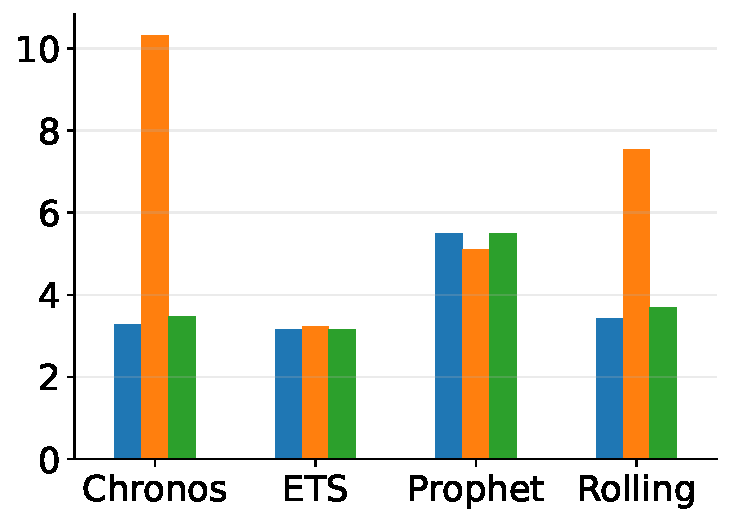
\includegraphics[width=\linewidth]
        {figures/m3_multi_prior_mape_percent.pdf}
        \caption{M3}
    \end{subfigure}\hfill
    \begin{subfigure}[t]{0.32\textwidth}
        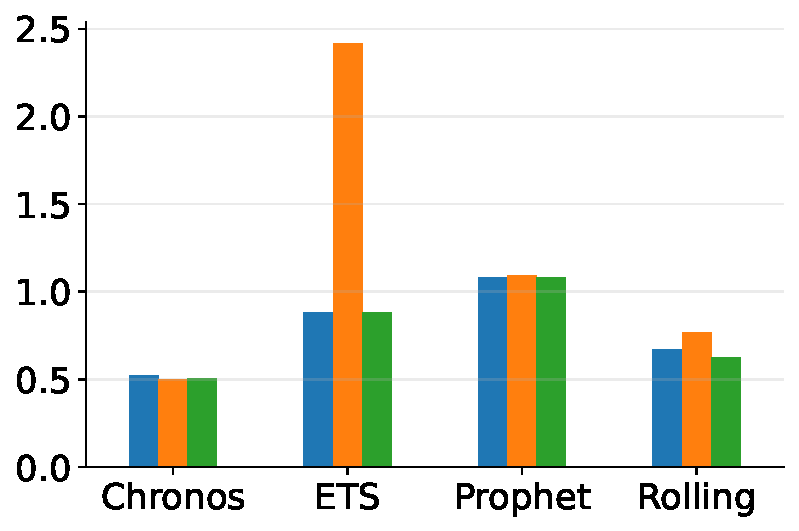
\includegraphics[width=\linewidth]
        {figures/ICMD_Dataset_multi_prior_mape_percent.pdf}
        \caption{ICMD}
    \end{subfigure}

    \medskip
    \begin{subfigure}[t]{0.32\textwidth}
        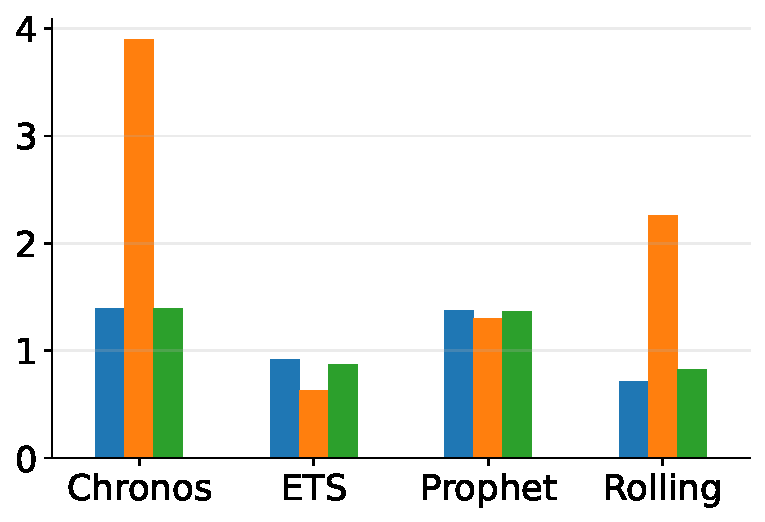
\includegraphics[width=\linewidth]
        {figures/tourism_multi_prior_mape_percent.pdf}
        \caption{Tourism}
    \end{subfigure}\hfill
    \begin{subfigure}[t]{0.32\textwidth}
        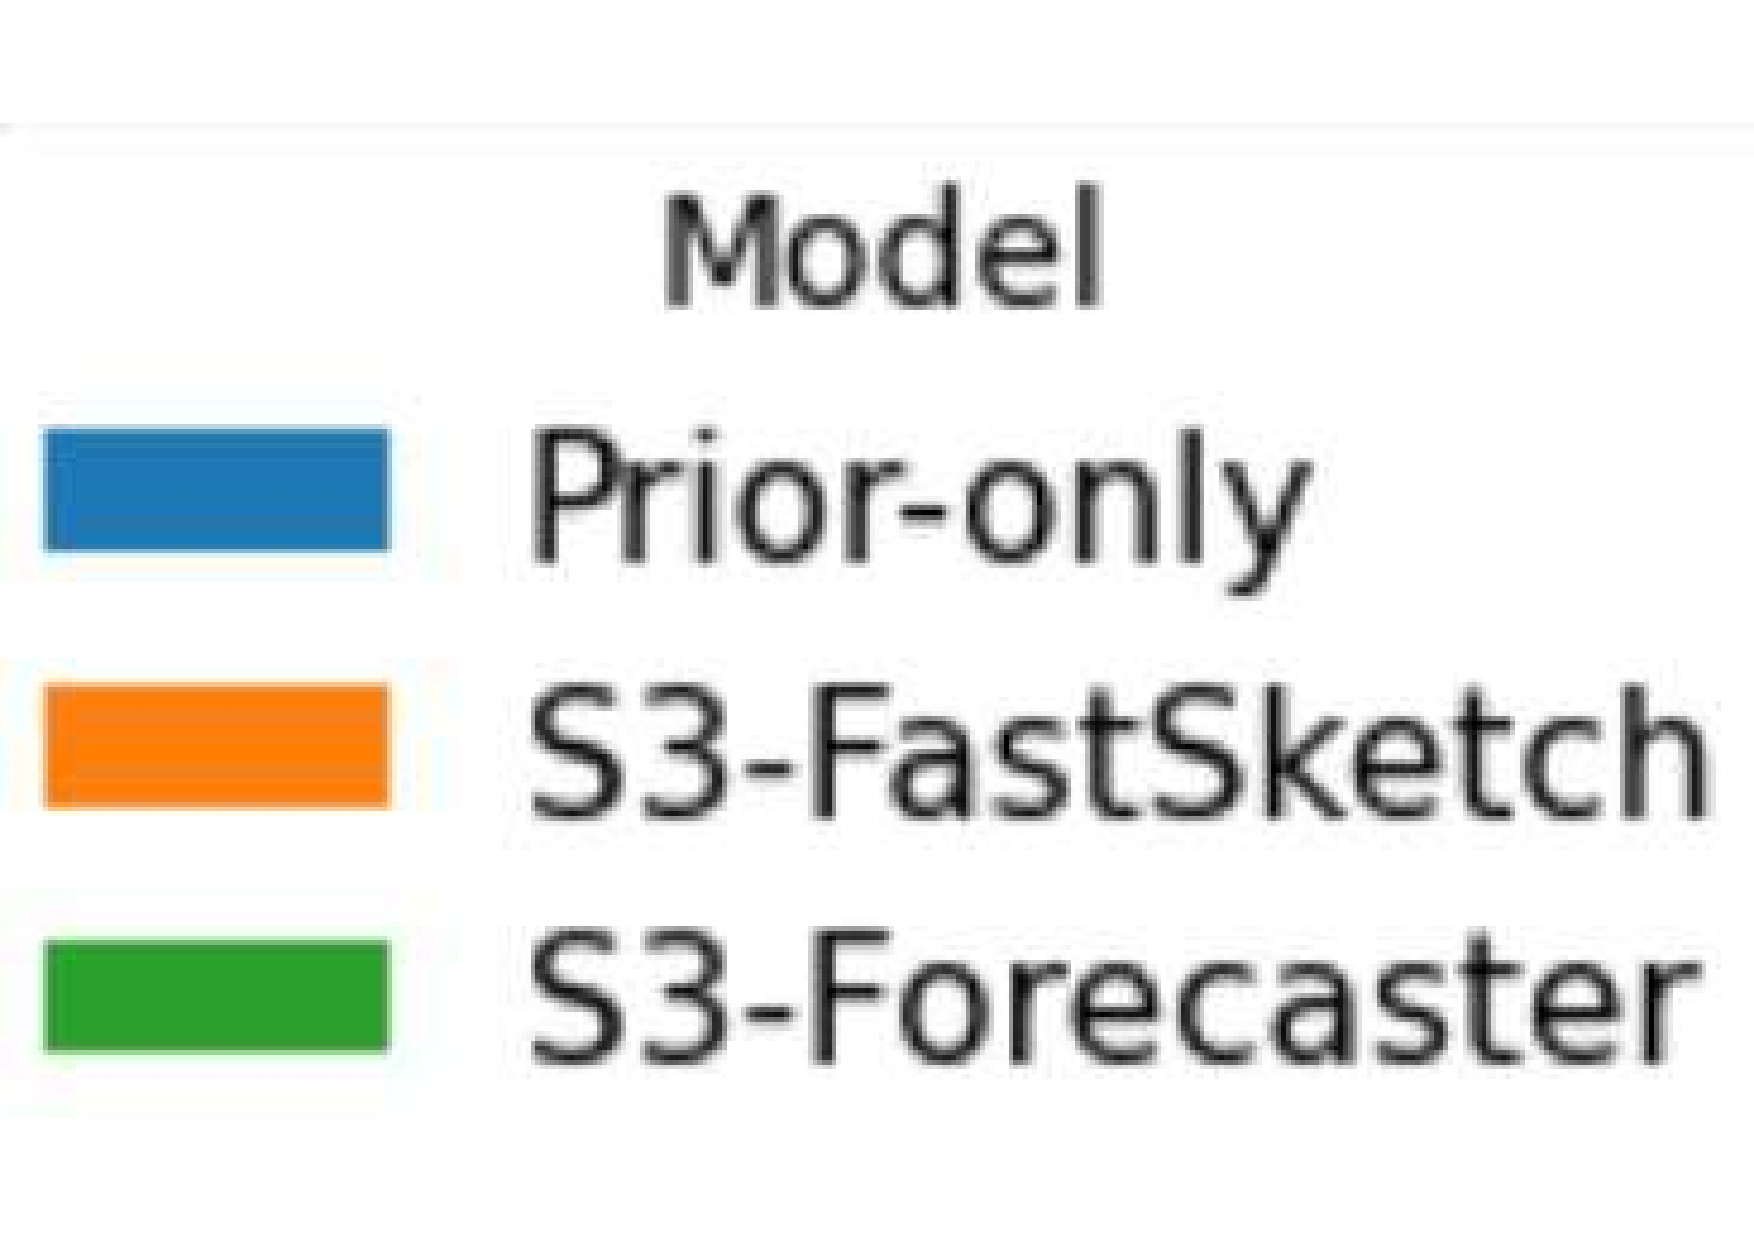
\includegraphics[width=\linewidth]
        {figures/modelos_multiprior.pdf}
        \caption{Model colors}
    \end{subfigure}\hfill
    \begin{subfigure}[t]{0.32\textwidth}
        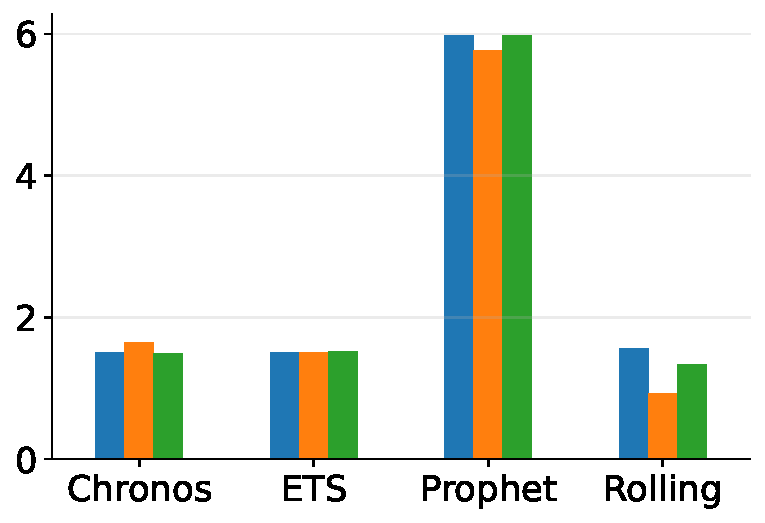
\includegraphics[width=\linewidth]
        {figures/M4_multi_prior_mape_percent.pdf}
        \caption{M4}
    \end{subfigure}
    \caption{Multi-prior transferability. The vertical axis reports MAPE as a percentage for each model--prior configuration.}
    \label{fig:multi_prior_all_datasets}
\end{figure*}

\subsection{Operational Efficiency and Parameter Economy}
\label{subsec:efficiency_results}

The operational-efficiency columns in Table~\ref{tab:uq_performance_vertical} report runtime after the stored dataset-level configurations have been loaded. On the model-scale benchmark, S3-Forecaster has a median
runtime of approximately $0.55$~s and a median of 802 trainable coefficients.
Across datasets with successful paired executions, the median runtime ratios
relative to S3-Forecaster are approximately $21\times$ for LSTM,
$9\times$ for CNN, and $5\times$ for AR-KAN. Chronos has zero target-trainable
coefficients in this accounting, but its median operational runtime is still
about $2.5\times$ that of S3-Forecaster.

S3-Forecaster is not the smallest or fastest model in absolute terms. Chronos,
AR, Kernel Ridge, ETS, and EasyTSF can require fewer learned coefficients or
lower latency in specific settings. Its engineering advantage is instead the
joint profile of nonlinear fixed-state representation, moderate target-domain
complexity, convex readout estimation, and the absence of iterative
backpropagation through the feature extractor. Because fixed reservoir matrices
and frozen prior parameters are excluded from the trainable-parameter count, the
parameter column measures statistical adaptation complexity rather than total
memory footprint.



\begin{figure}[t]
    \centering
    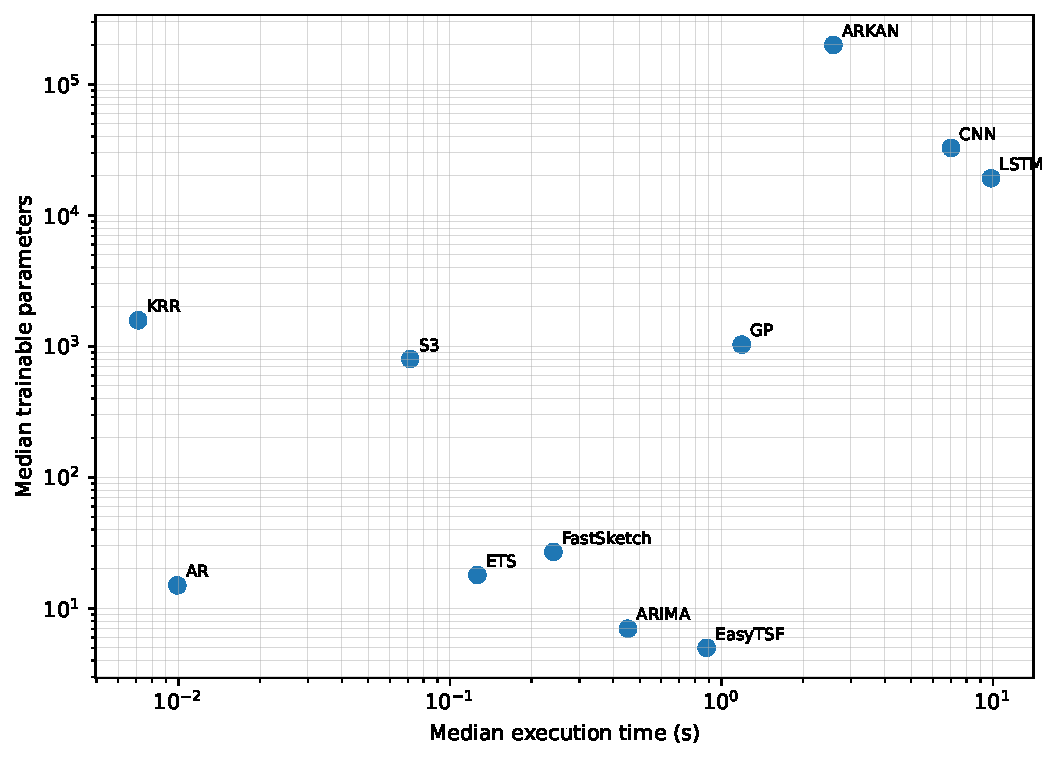
\includegraphics[width=0.94\linewidth]
    {figures/runtime_parameter_tradeoff.pdf}
    \caption{Operational runtime--parameter trade-off.}
    \label{fig:runtime_parameter_tradeoff}
\end{figure}

\subsection{Limitations and Scientific Synthesis}
\label{subsec:scientific_synthesis}

The complete evidence supports a selective rather than universal interpretation
of the S3 family. ICMD remains the principal engineering case: S3-Forecaster
achieves the strongest model-scale RMSE and $R^2$, S3-FastSketch gives the best
proportional point error, and Chronos gives the best interval score. This split
shows that point accuracy, proportional error, and interval efficiency can favor
different mechanisms even on the same industrial series.

M4 provides the principal reproducible public result for the S3 family:
S3-FastSketch is strongest in point forecasting, while S3-Forecaster gives the
best adaptive conformal MSIS. CIF supports the value of the larger reservoir,
whereas Tourism favors the compact sketch representation. M3 remains a boundary
case in which S3-Forecaster ties ETS in point metrics but under-covers in
adaptive conformal evaluation. 

% The contribution should therefore be stated as an engineering adaptation
% mechanism rather than a universally superior forecaster. After a one-time
% dataset-level HPO stage, S3-Forecaster provides rapid operational fitting and
% forecasting without end-to-end gradient optimization. Its benefit is greatest
% when the frozen prior leaves a stable, conditionally predictable residual
% component. When that condition is not met, the unadapted prior, a parsimonious
% statistical model, or S3-FastSketch may be preferable.

% This interpretation aligns the evidence with the intended EAAI narrative:
% \begin{equation}
% \boxed{
% \begin{array}{c}
% \text{short industrial histories}
% \\[-1mm]
% +\ \text{gradient-free residual adaptation}
% \\[-1mm]
% +\ \text{adaptive conformal uncertainty estimation}
% \\[-1mm]
% +\ \text{public reproducible validation}
% \\[-1mm]
% +\ \text{low operational cost}
% \end{array}
% }
% \end{equation}
% The results substantiate engineering relevance and methodological
% promise under non-stationary small-data conditions, while explicitly delimiting
% the cases in which residual adaptation and interval estimation remain
% unreliable.

\FloatBarrier
